\section{Detection results}
\label{sec:results}

\subsection{Evaluation protocol}

Every system is scored by the same code, tested against scikit-learn:
\begin{itemize}
  \item \textbf{LexGLUE micro-F1 and macro-F1}, with the ``8+1'' convention of LexGLUE~\citep{chalkidis2022lexglue}: a ninth \emph{fair} label is added, so that our numbers are comparable with published ones;
  \item \textbf{precision and recall of unfair sentences}, i.e.\ any category against fair: the quantities that matter for a consumer;
  \item \textbf{per-category} precision, recall and F1, with the number of test sentences;
  \item \textbf{95\% bootstrap confidence intervals}~\citep{efron1993} with 1,000 resamples of the test sentences, because some categories have very few examples.
\end{itemize}
To decide whether two systems really differ, we use a paired bootstrap~\citep{bergkirkpatrick2012}: the same resampled sentences score both systems, and a difference is significant at 5\% when its 95\% interval excludes zero.

\subsection{Main results}

Table~\ref{tab:main} and Figure~\ref{fig:main} give the results on the 1,607 test sentences. Table~\ref{tab:significance} tests the differences between the main system and the others.

\begin{table}[ht]
\centering\small
\caption{Results on the UNFAIR-ToS test set (1,607 sentences, 172 unfair). Legal-BERT: mean $\pm$ standard deviation over three seeds. The main system was declared before its test run.}
\label{tab:main}
\begin{tabular}{@{}lrrrr@{}}
\toprule
System & Micro-F1 & Macro-F1 & Precision & Recall \\
\midrule
Always fair & 88.9 & 10.5 & 0.0 & 0.0 \\
TF-IDF + SVM & 95.4 & 78.6 & 91.5 & 69.2 \\
kNN vote (bge-m3, $k=3$, $t=2$) & 94.8 & 77.8 & 78.0 & 82.6 \\
Plain LLM (gpt-4.1-mini, zero-shot) & 84.0 & 64.2 & 41.3 & 93.6 \\
Legal-BERT, fine-tuned & 95.9 $\pm$ 0.4 & 82.7 $\pm$ 1.1 & 85.7 $\pm$ 4.4 & 82.0 $\pm$ 3.5 \\
RAG, no gate & 90.2 & 71.3 & 55.0 & 93.0 \\
RAG examples only + gate & 95.6 & 78.9 & 83.7 & 80.8 \\
\textbf{RAG + evidence gate (main)} & \textbf{95.6} & \textbf{79.4} & \textbf{82.3} & \textbf{83.7} \\
\midrule
TF-IDF + SVM, LexGLUE paper & 94.7 & 75.0 & -- & -- \\
Legal-BERT, LexGLUE paper & 96.0 & 83.0 & -- & -- \\
\bottomrule
\end{tabular}
\end{table}

\begin{figure}[ht]
\centering
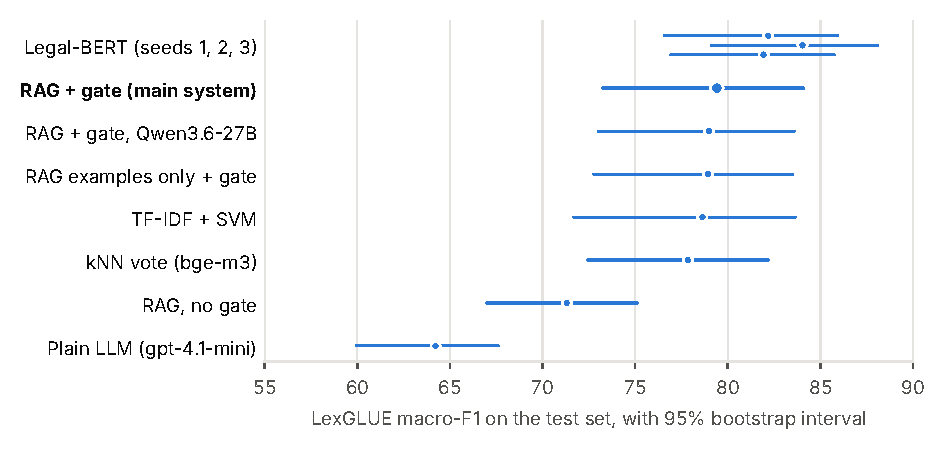
\includegraphics[width=0.82\textwidth]{test_macro_f1.pdf}
\caption{Test macro-F1 with 95\% bootstrap intervals. The intervals of the main system, Legal-BERT, TF-IDF and the kNN vote overlap widely.}
\label{fig:main}
\end{figure}

\begin{table}[ht]
\centering\small
\caption{Paired bootstrap on the test set: the main system minus each other system (1,000 resamples). $^{*}$ significant at 5\%.}
\label{tab:significance}
\begin{tabular}{@{}lrrr@{}}
\toprule
Main system minus\ldots & Macro-F1 & Precision & Recall \\
\midrule
Legal-BERT, seeds 1 / 2 / 3 & $-$2.5 / $-$4.6 / $-$2.8 & +0.4 / $-$8.3$^{*}$ / $-$2.4 & $-$0.6 / +5.8 / 0.0 \\
TF-IDF + SVM & +0.8 & $-$9.3$^{*}$ & +14.5$^{*}$ \\
kNN vote & +1.6 & +4.3 & +1.2 \\
Plain LLM & +15.2$^{*}$ & +41.0$^{*}$ & $-$9.9$^{*}$ \\
RAG, no gate & +8.1$^{*}$ & +27.3$^{*}$ & $-$9.3$^{*}$ \\
RAG examples only + gate & +0.5 & $-$1.4 & +2.9$^{*}$ \\
\bottomrule
\end{tabular}
\end{table}

\paragraph{The baselines fail in different ways.}
\begin{itemize}
  \item \textbf{TF-IDF} is precise but misses almost one unfair clause in three.
  \item \textbf{The plain LLM} finds 93.6\% of the unfair clauses but flags 390 sentences for 172 unfair ones. Most of its false alarms are sentences on the \emph{topic} of an unfair clause. For example, 72 of its 77 false arbitration alarms are procedural sentences within about 50 sentences of an arbitration clause, and some of them even protect the consumer.
  \item \textbf{Legal-BERT} reproduces the published result (82.7 against 83.0 macro-F1) and has the best balance, but it misses about one unfair clause in five and gives no reasons.
\end{itemize}

\paragraph{The main system matches the best baselines and explains every flag.} With 79.4 macro-F1, the RAG system with the evidence gate is statistically on par with Legal-BERT, TF-IDF and the kNN vote. Legal-BERT keeps a lead of 2.5--4.6 points that this test set, with 7 to 38 sentences per category, cannot confirm. The main system finds 14.5 points more unfair clauses than TF-IDF, and it is clearly better than the plain LLM and than RAG without the gate. The gate is the decisive step: it adds 8.1 macro-F1 and 27.3 precision for a loss of 9.3 points of recall. What the main system adds over all baselines is the explanation. Of its 175 flags, 95.4\% cite a specific legal rationale or provision, 65.7\% a specific article, Annex point or court judgment, and 77.7\% the expert precedents they resemble; no cited id was invented. The most cited sources, apart from the general test of Article 3(1), are Annex points 1(j) and 1(k) of the Directive (unilateral change of the terms and of the service), 1(i) and 1(q), and the \emph{Oc\'eano} judgment. The test run cost \$1.64.

\paragraph{Per category} (Table~\ref{tab:percategory}), jurisdiction and choice of law are almost always right when flagged. Arbitration is found (6 of 7) but with many false alarms, the same weakness as the plain LLM and the kNN vote: sentences of an arbitration section look alike whether they are unfair or not. Content removal is the weakest category, with 13 test sentences.

\begin{table}[ht]
\centering\small
\caption{Main system per category on the test set.}
\label{tab:percategory}
\begin{tabular}{@{}lrrrr@{}}
\toprule
Category & Test sentences & Precision & Recall & F1 \\
\midrule
Limitation of liability & 38 & 82 & 71 & 76 \\
Unilateral termination & 38 & 71 & 79 & 75 \\
Unilateral change & 38 & 81 & 79 & 80 \\
Contract by using & 23 & 79 & 83 & 81 \\
Content removal & 13 & 67 & 62 & 64 \\
Choice of law & 13 & 100 & 77 & 87 \\
Jurisdiction & 16 & 100 & 94 & 97 \\
Arbitration & 7 & 43 & 86 & 57 \\
\bottomrule
\end{tabular}
\end{table}

\subsection{Which knowledge helps?}
\label{sec:ablation}

Table~\ref{tab:ablation} varies the knowledge in the prompt on the validation set. The useful signal for detection comes from the expert-labelled examples. Legal knowledge alone makes the model flag even more sentences than with no retrieval: 493 false alarms instead of 338, mostly limitation of liability and arbitration. Reading descriptions of unfair practices primes the model to find them everywhere. Added to the examples, the legal knowledge still costs precision.

Yet the legal knowledge is what grounds the explanations in the law. In the full RAG, 95.5\% of the unfair verdicts cite a specific rationale or provision, while without it an explanation can only point to similar sentences. After the gate the two variants are within one point of macro-F1 on validation and on test (+0.5, not significant), and the legal knowledge adds 2.9 points of recall on test (significant). We kept the full RAG with the gate as the main system, declared before the test run.

\begin{table}[ht]
\centering\small
\caption{Ablation on validation (2,275 sentences, 230 unfair): knowledge in the prompt.}
\label{tab:ablation}
\begin{tabular}{@{}lrrrrr@{}}
\toprule
Knowledge in the prompt & Macro-F1 & Precision & Recall & False alarms & With gate: macro-F1 \\
\midrule
None (plain LLM) & 60.8 & 38.5 & 92.2 & 338 & -- \\
Rationales and provisions only & 52.9 & 31.1 & 97.0 & 493 & -- \\
Examples only & 71.5 & 61.1 & 87.4 & 128 & 78.4 \\
Examples, rationales and provisions & 65.7 & 50.2 & 92.2 & 210 & 77.5 \\
\bottomrule
\end{tabular}
\end{table}
